\begin{figure}[!htb]
\centering
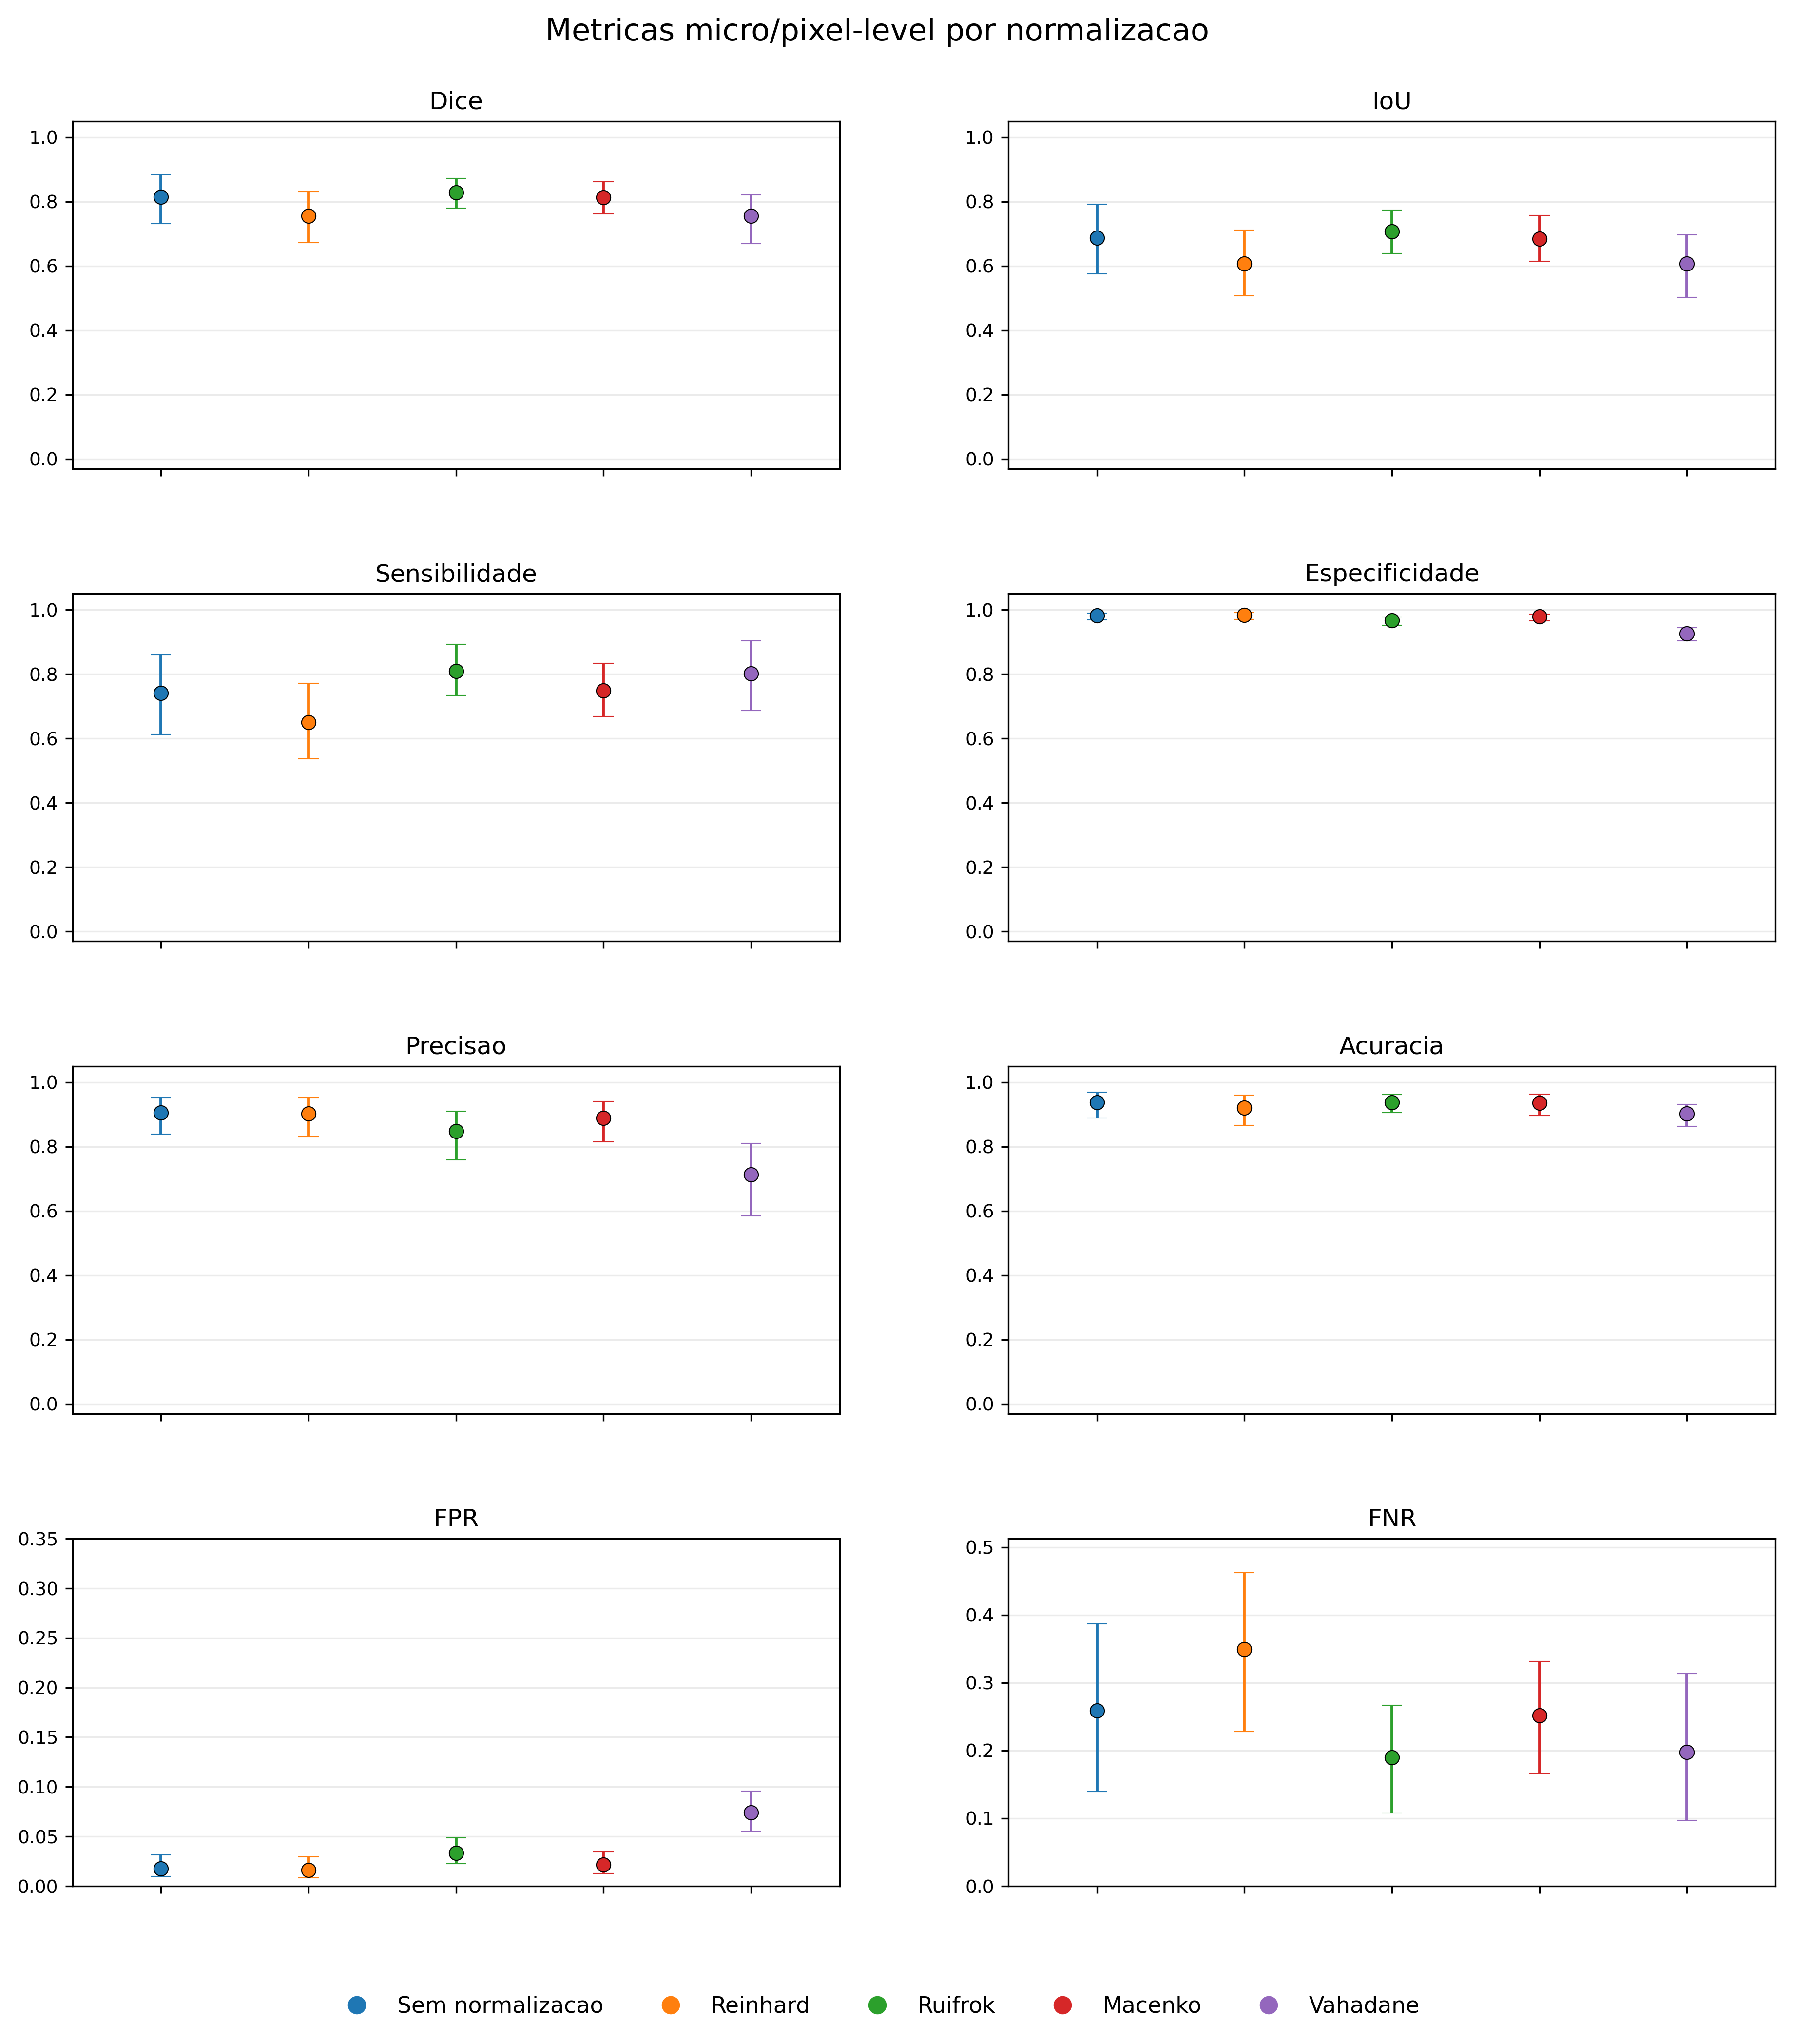
\includegraphics[width=0.98\textwidth,height=0.86\textheight,keepaspectratio]{figuras/results_diagset_micro_metrics.png}
\caption{Metricas micro no conjunto de teste de DIAGSET.}
\label{fig:results_diagset-micro-metrics}
\end{figure}

\begin{figure}[!htb]
\centering
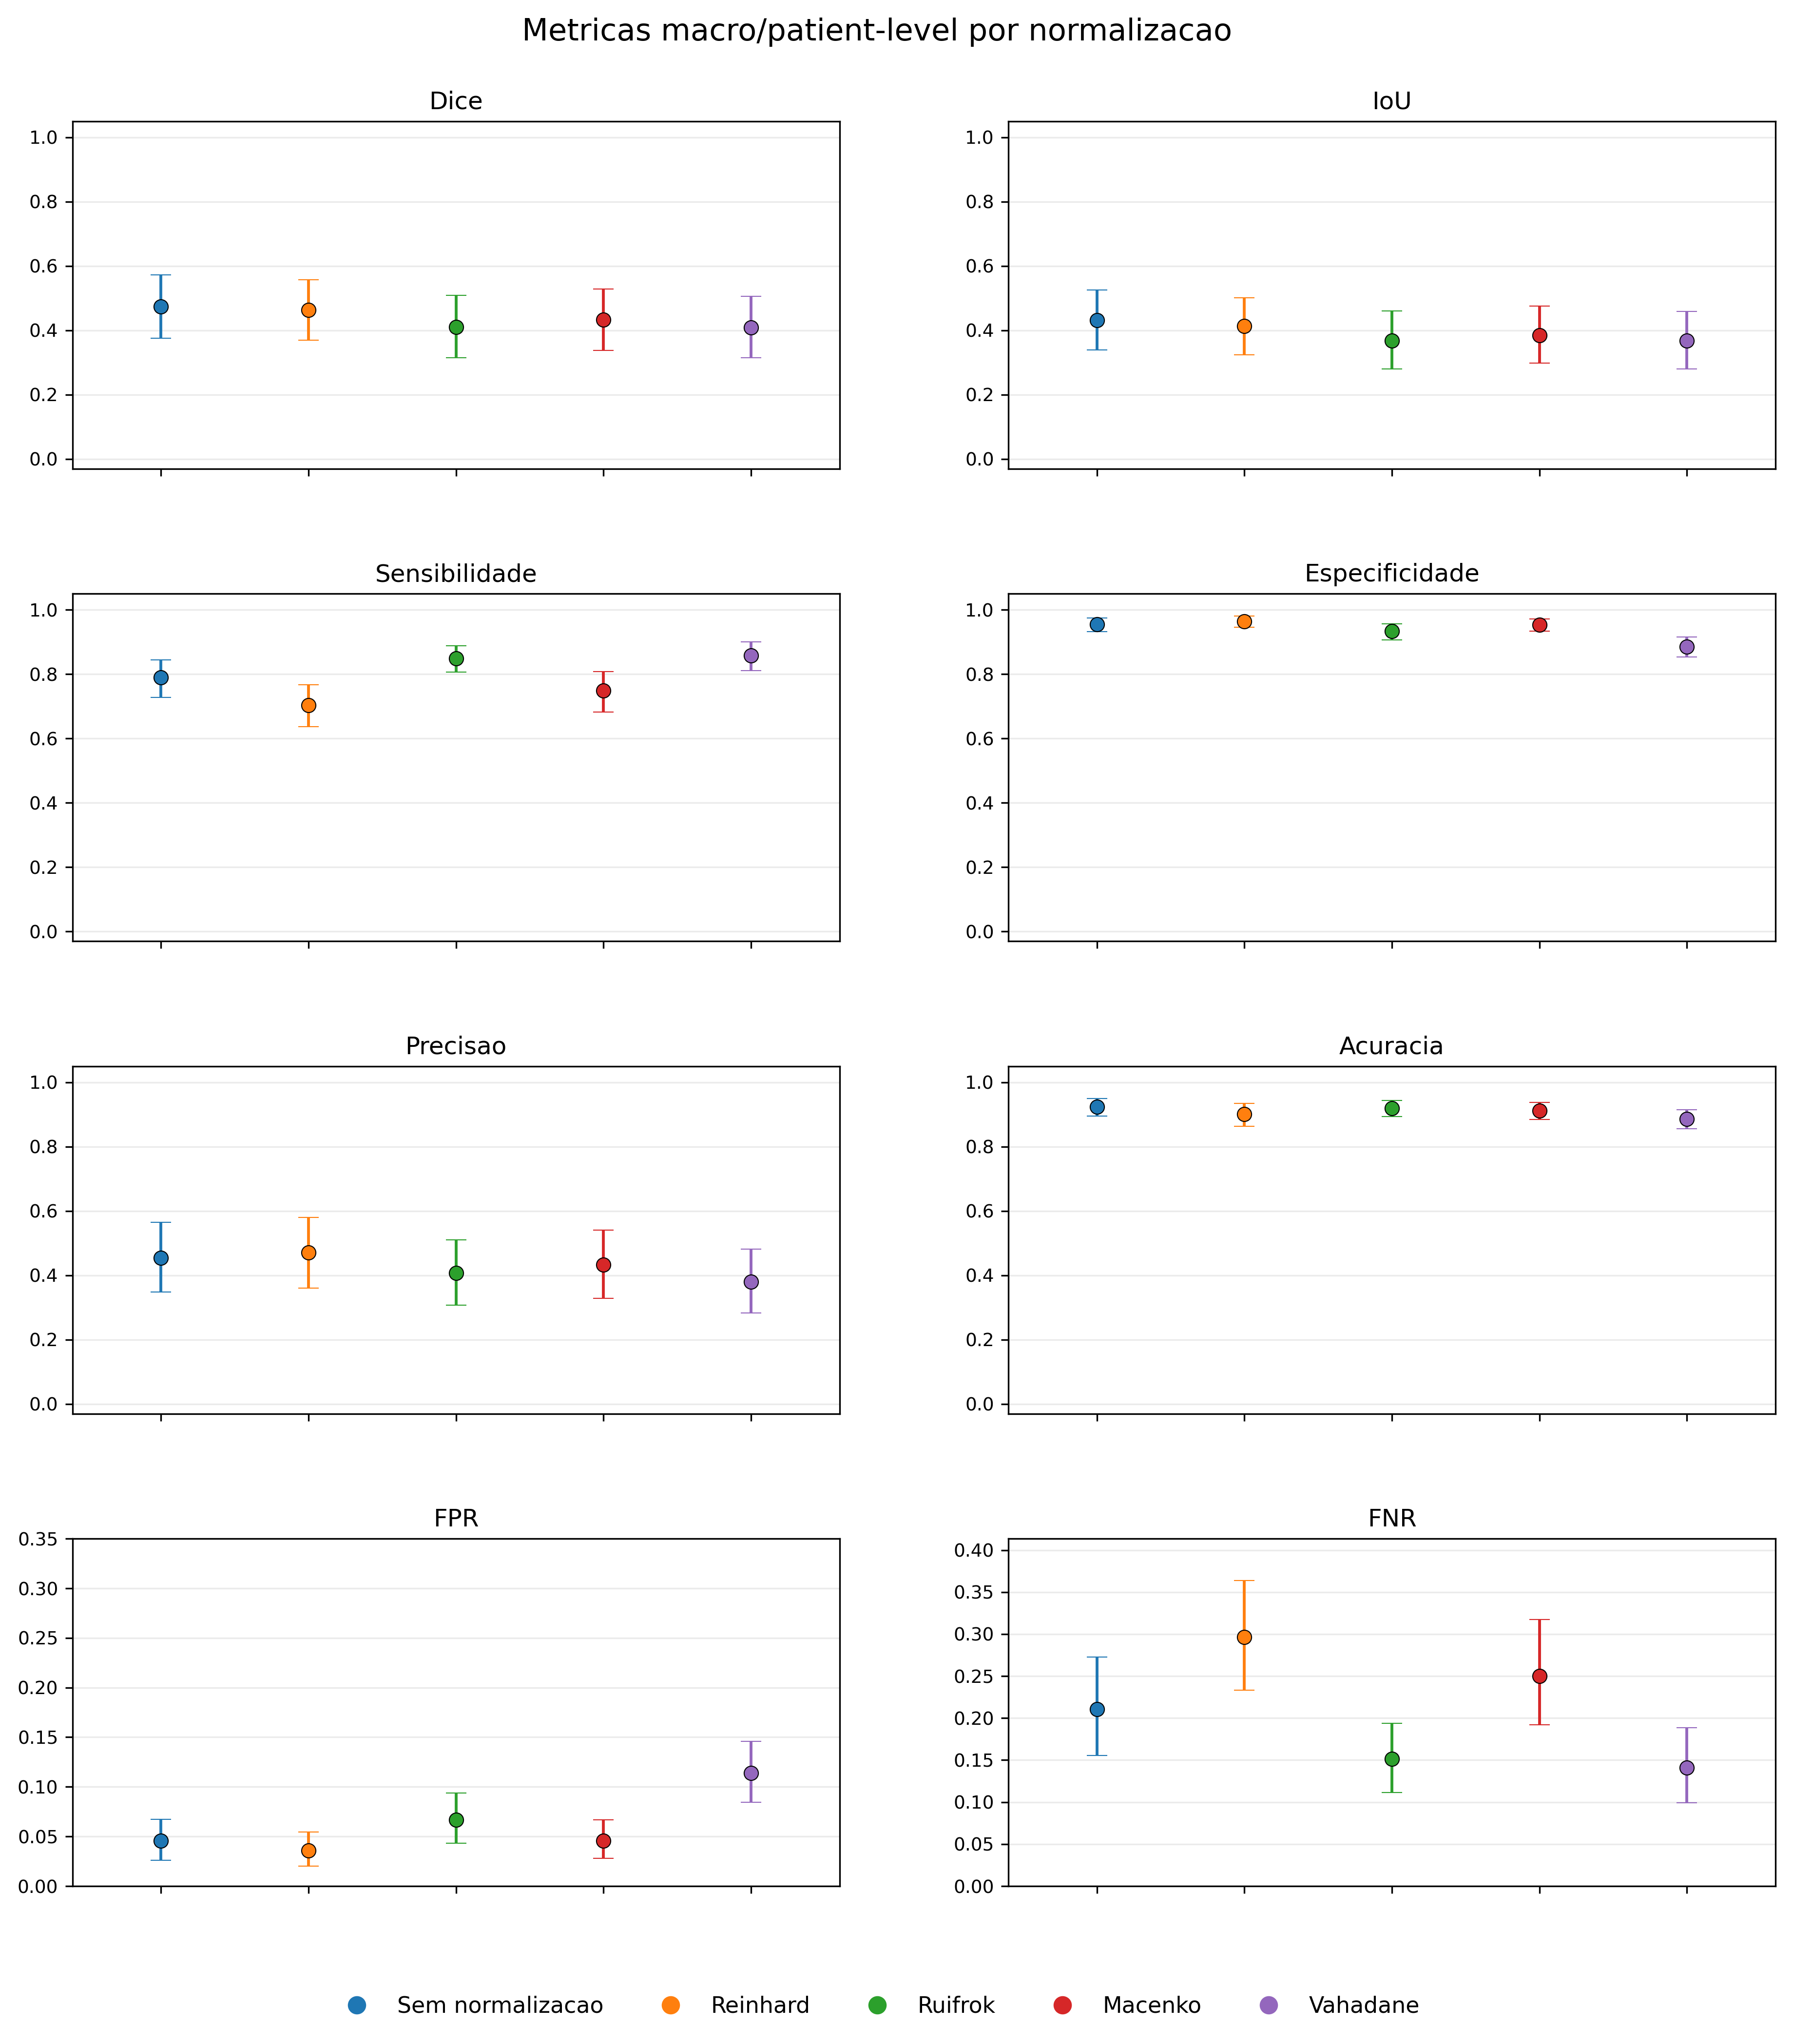
\includegraphics[width=0.98\textwidth,height=0.86\textheight,keepaspectratio]{figuras/results_diagset_macro_metrics.png}
\caption{Metricas macro por paciente no conjunto de teste de DIAGSET.}
\label{fig:results_diagset-macro-metrics}
\end{figure}

\begin{figure}[!htb]
\centering
\begin{subfigure}[t]{0.48\textwidth}
\centering
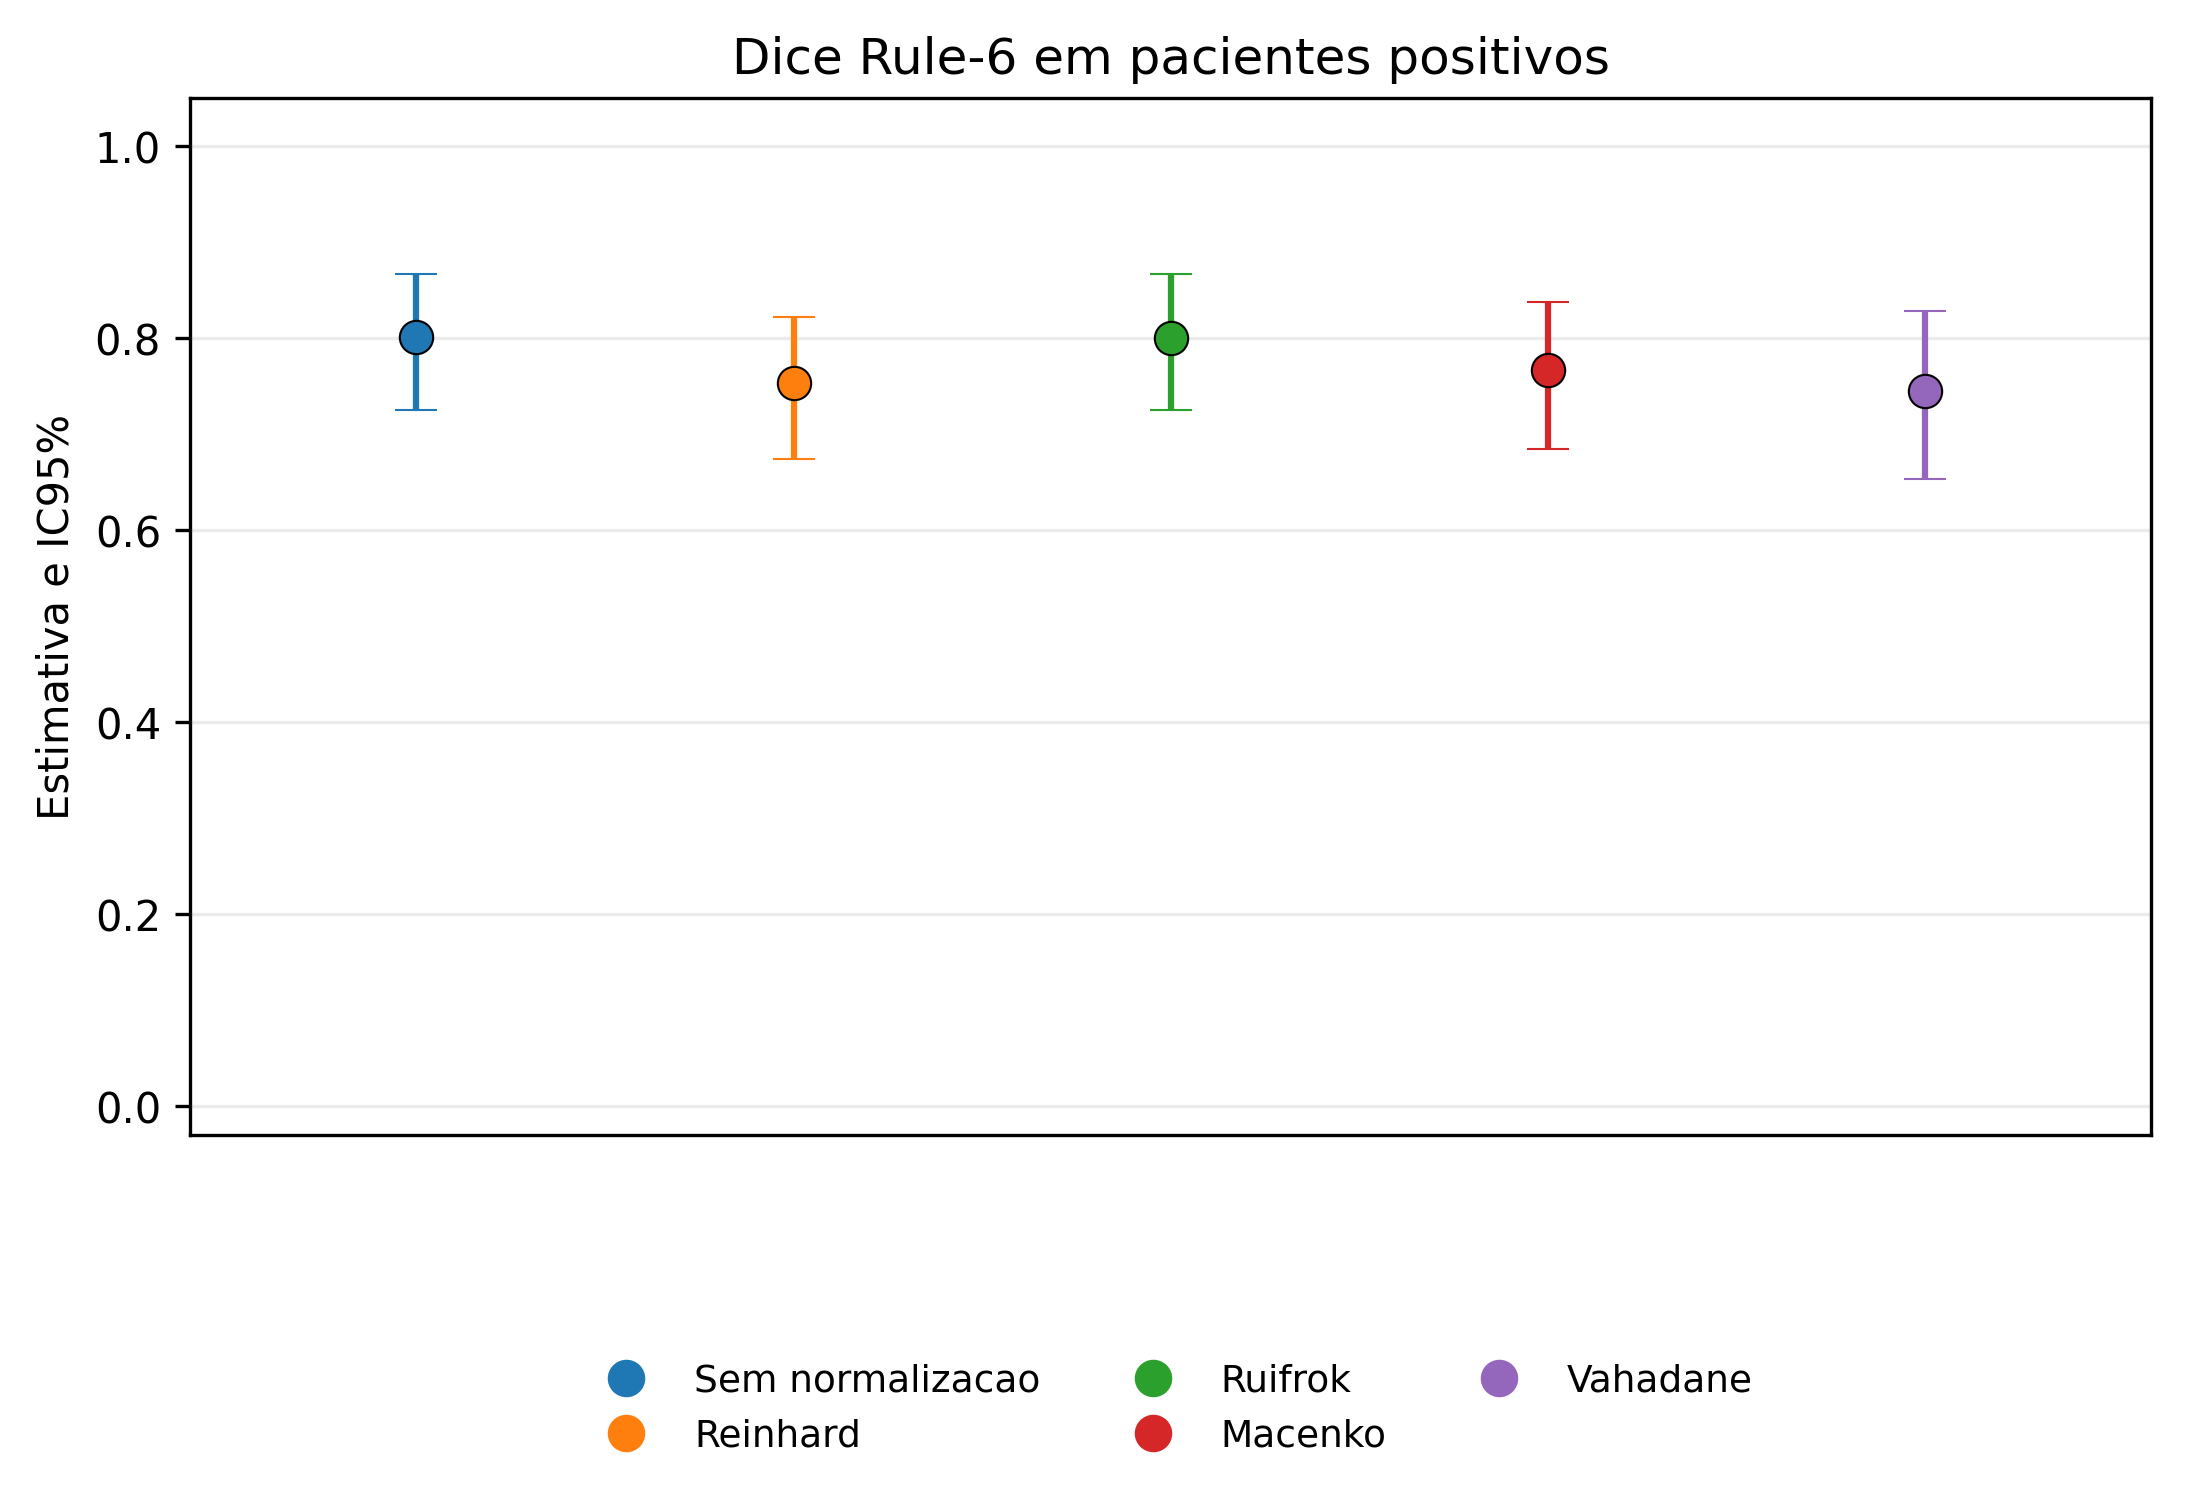
\includegraphics[width=\linewidth]{figuras/results_diagset_rule6_dice_pos.png}
\caption{Dice em pacientes positivos}
\label{fig:results_diagset-rule6-dice-pos}
\end{subfigure}
\hfill
\begin{subfigure}[t]{0.48\textwidth}
\centering
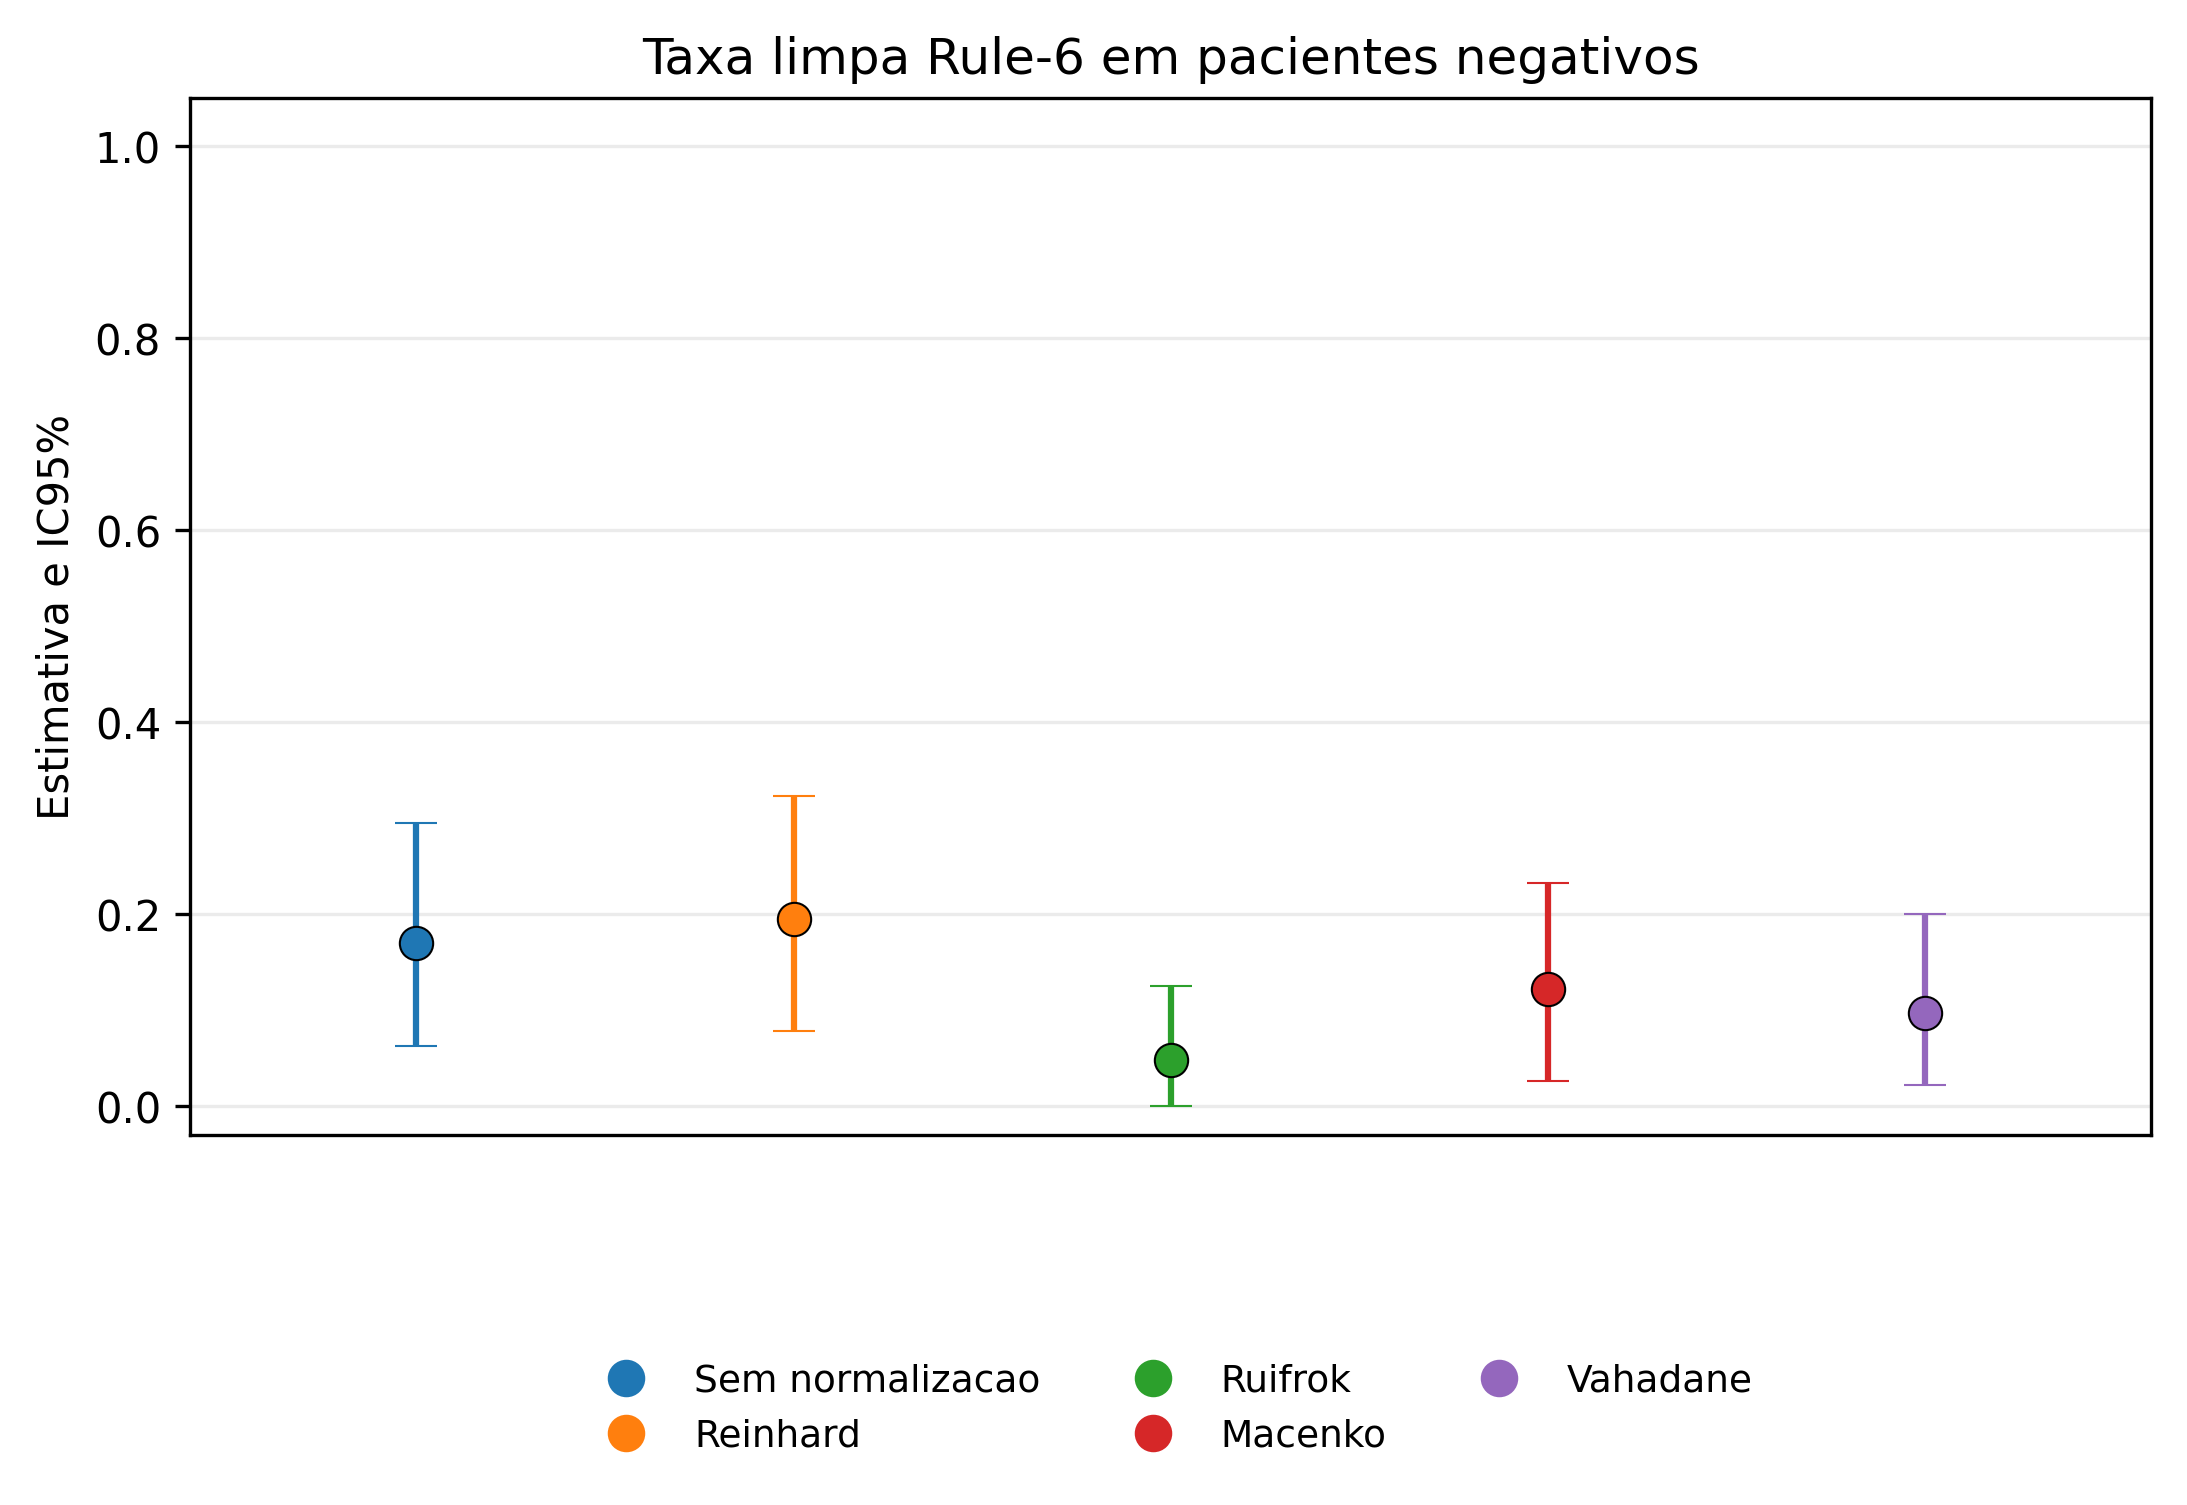
\includegraphics[width=\linewidth]{figuras/results_diagset_rule6_neg_clean.png}
\caption{Taxa limpa em pacientes negativos}
\label{fig:results_diagset-rule6-neg-clean}
\end{subfigure}
\caption{Metricas Rule-6 no conjunto de teste de DIAGSET.}
\label{fig:results_diagset-rule6-metrics}
\end{figure}

\begin{figure}[!htb]
\centering
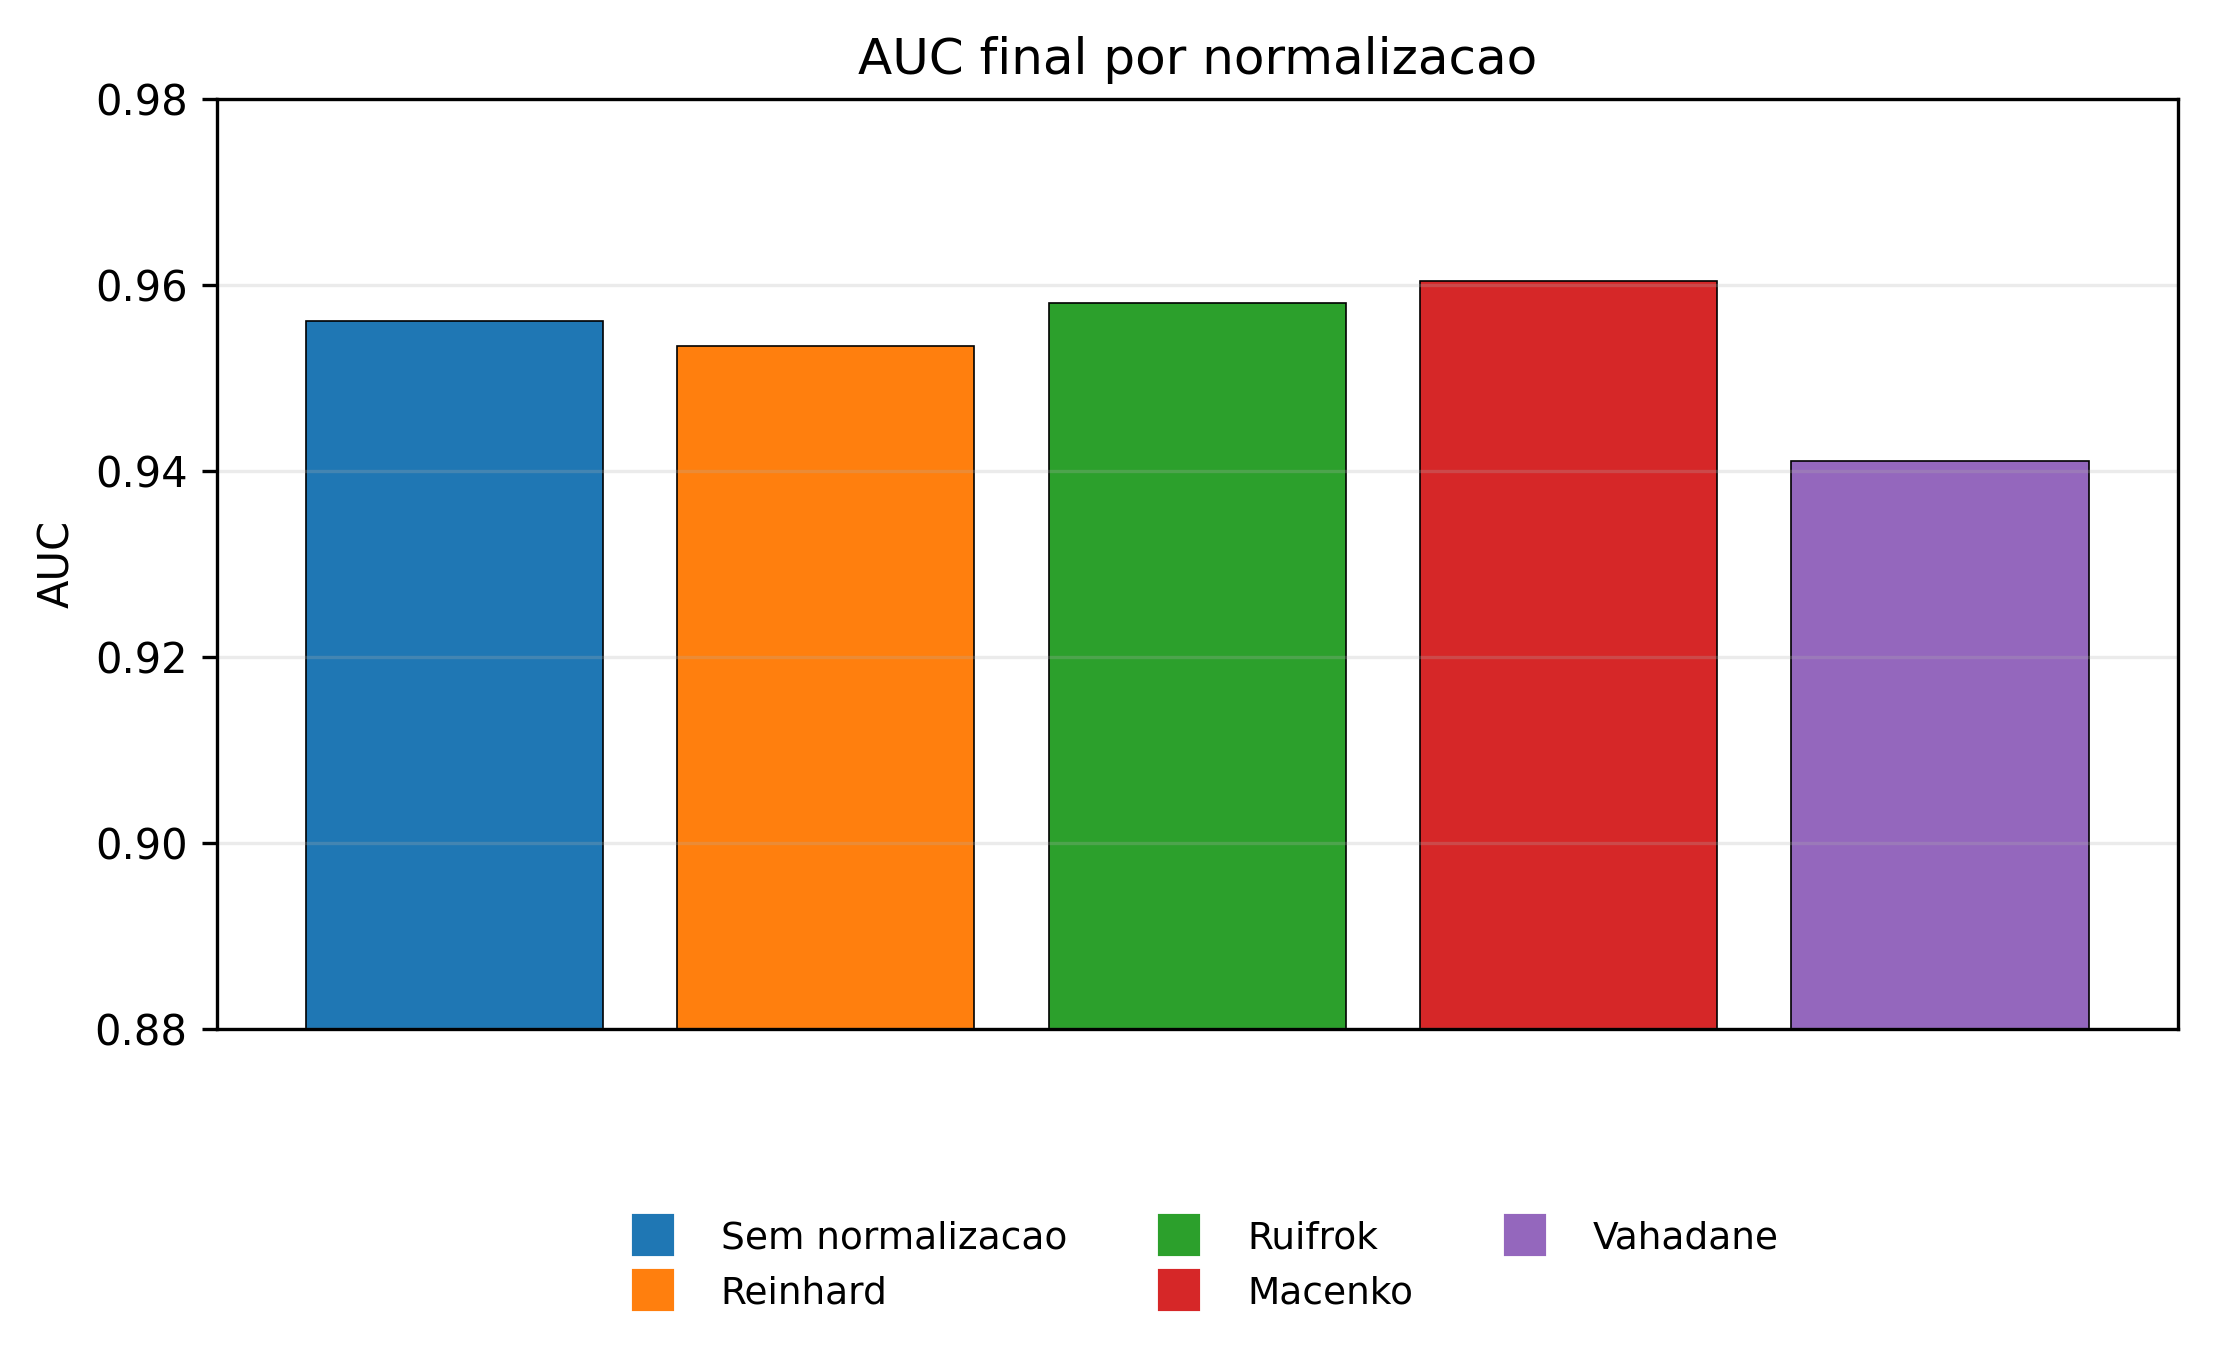
\includegraphics[width=0.94\textwidth]{figuras/results_diagset_auc_thresholds.png}
\caption{AUC no conjunto de teste de DIAGSET.}
\label{fig:results_diagset-auc-thresholds}
\end{figure}

\begin{figure}[!htb]
\centering
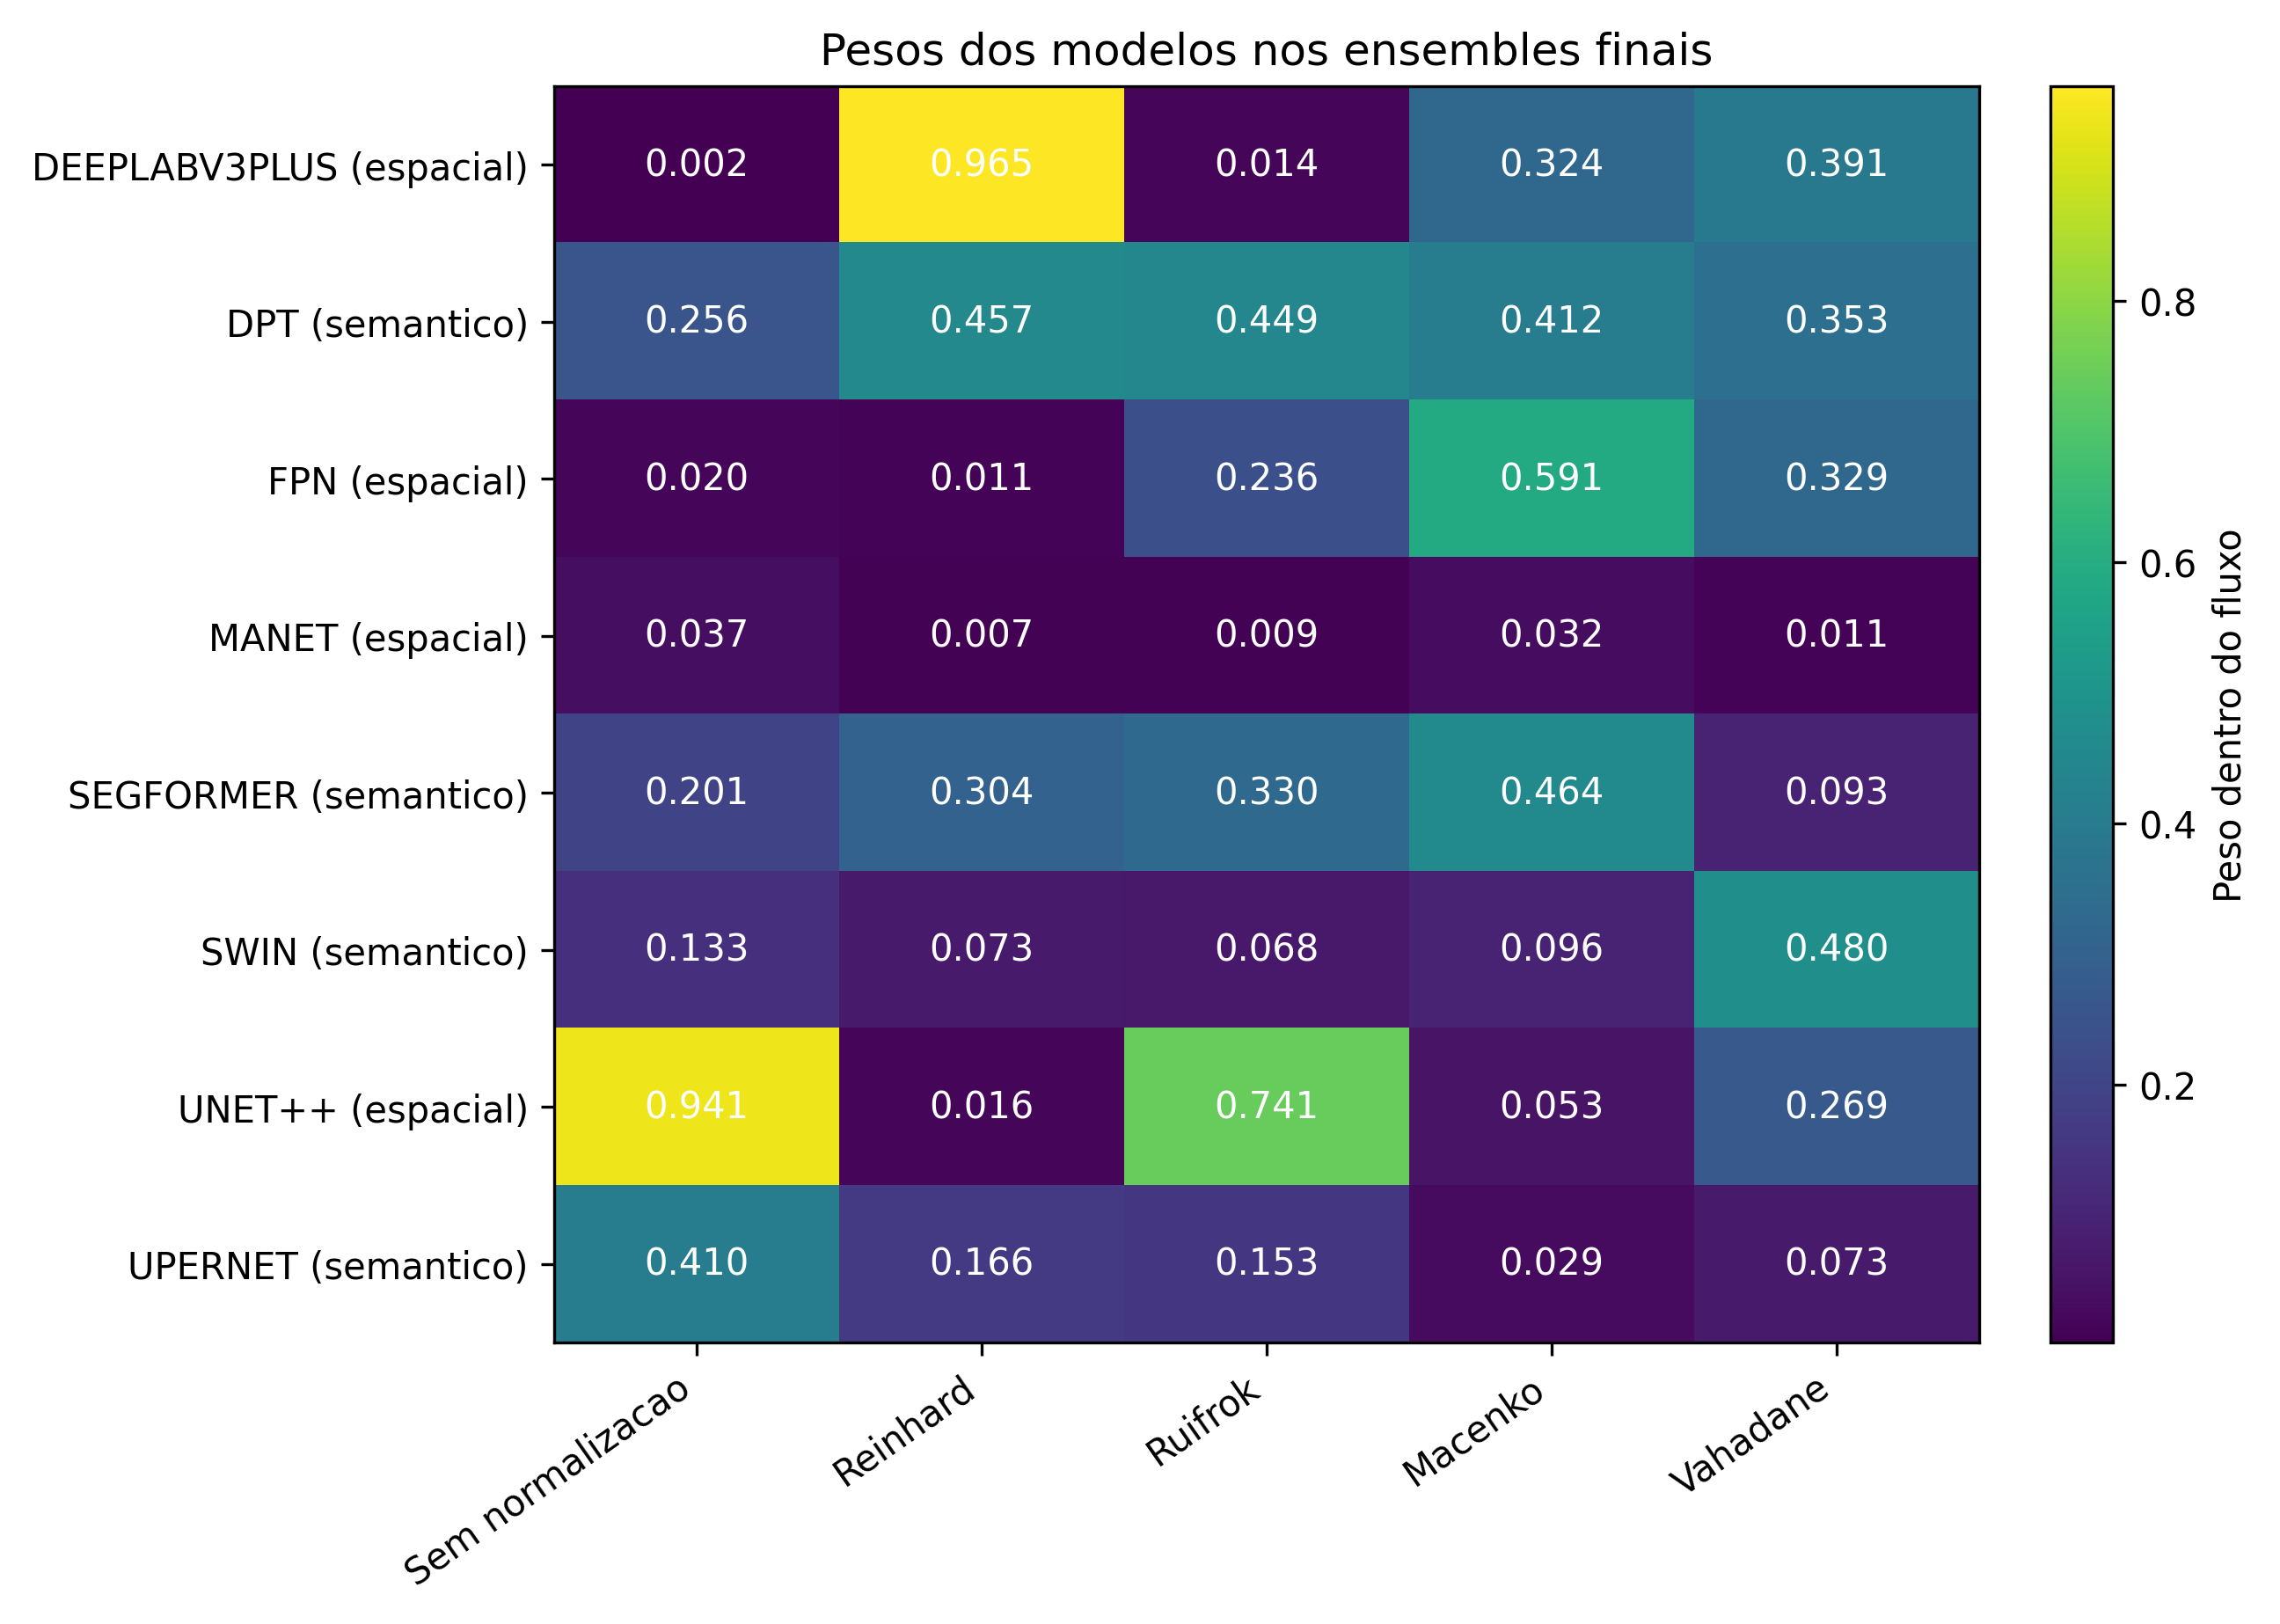
\includegraphics[width=0.94\textwidth]{figuras/results_diagset_ensemble_weights.png}
\caption{Pesos dos modelos nos ensembles finais de DIAGSET.}
\label{fig:results_diagset-ensemble-weights}
\end{figure}
